\section{Triangular}

\begin{figure}[h]
\centering
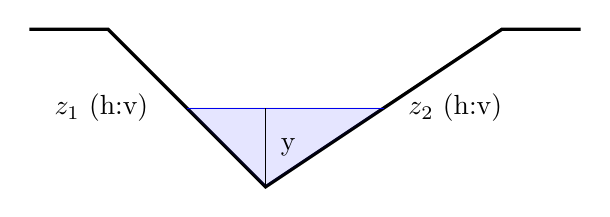
\begin{tikzpicture}
\draw[very thick] (0,0) -- (1,0) -- node[left=10pt]{$z_1$ (h:v)}(3,-2)--node[right=5]{$z_2$ (h:v)} (6,0) -- (7,0);
\draw[blue] (2,-1) -- (4.5,-1);

\filldraw[fill=blue, opacity=0.1](2, -1) --(4.5, -1) -- (3, -2);


\draw (3,-2)--node[right=2]{y} (3,-1);
\end{tikzpicture}
\caption{Triangular Section}
\end{figure}

\begin{equation}
A = \frac{1}{2} (z_1 + z_2) y^2
\end{equation}

\begin{equation}
P = \left(\sqrt{1+z_1^2} + \sqrt{1+z_2^2}\right)y
\end{equation}

\begin{equation}
R = \frac{1}{2}\frac{(z_1 + z_2) }{\sqrt{1+z_1^2} + \sqrt{1+z_2^2}}y
\end{equation}
Eq. (\ref{Eq:Q}) becomes
\begin{equation}
Q = \frac{K_u}{n} \frac{z_1 + z_2}{2}  \left(\frac{1}{2}\frac{z_1 + z_2}{\sqrt{1+z_1^2} + \sqrt{1+z_2^2}}\right)^{\frac{2}{3}} y^{\frac{8}{3}}S^{\frac{1}{2}}.
\end{equation}
Note this equation can be used to backcalculate $y$ from $Q$.
\begin{equation}
\frac{\partial A}{\partial y} = (z_1 + z_2)y
\end{equation}
Eq. (\ref{Eq:C}) becomes
\begin{equation}  
f_c(y)= \frac{g}{8}(z_1 + z_2)^3y^6 - Q^2(z_1 + z_2)y = 0.
\end{equation}

\begin{equation}  
y_c^5 = \frac{8Q^2}{g(z_1 + z_2)^2}
\end{equation}

